\begin{equation}
    - \Sigma = \begin{gathered}
        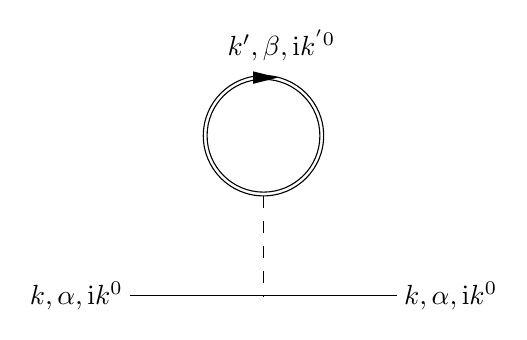
\begin{tikzpicture}[x=0.75pt,y=0.75pt,yscale=-1,xscale=1]
            %uncomment if require: \path (0,300); %set diagram left start at 0, and has height of 300
            
            %Straight Lines [id:da21065414652163694] 
            \draw    (226.85,232) -- (355.85,232) ;
            %Straight Lines [id:da10375589245043493] 
            \draw  [dash pattern={on 4.5pt off 4.5pt}]  (291.35,183.98) -- (291.35,232) ;
            %Shape: Circle [id:dp49575130445920723] 
            \draw   (262.35,154.98) .. controls (262.35,138.96) and (275.34,125.98) .. (291.35,125.98) .. controls (307.37,125.98) and (320.35,138.96) .. (320.35,154.98) .. controls (320.35,171) and (307.37,183.98) .. (291.35,183.98) .. controls (275.34,183.98) and (262.35,171) .. (262.35,154.98) -- cycle ;
            %Straight Lines [id:da49696357001991487] 
            \draw    (298.35,126.98) ;
            \draw [shift={(298.35,126.98)}, rotate = 180] [fill={rgb, 255:red, 0; green, 0; blue, 0 }  ][line width=0.08]  [draw opacity=0] (12,-3) -- (0,0) -- (12,3) -- cycle    ;
            %Shape: Circle [id:dp3232390185153] 
            \draw   (264.18,154.98) .. controls (264.18,139.97) and (276.34,127.8) .. (291.35,127.8) .. controls (306.36,127.8) and (318.53,139.97) .. (318.53,154.98) .. controls (318.53,169.99) and (306.36,182.16) .. (291.35,182.16) .. controls (276.34,182.16) and (264.18,169.99) .. (264.18,154.98) -- cycle ;
            
            % Text Node
            \draw (224.85,232) node [anchor=east] [inner sep=0.75pt]    {$\boldsymbol{k} ,\alpha ,\mathrm{i} k^{0}$};
            % Text Node
            \draw (357.85,232) node [anchor=west] [inner sep=0.75pt]    {$\boldsymbol{k} ,\alpha ,\mathrm{i} k^{0}$};
            % Text Node
            \draw (327.17,111.51) node [anchor=east] [inner sep=0.75pt]    {$\boldsymbol{k} ',\beta ,\mathrm{i} k^{'0}$};
            \end{tikzpicture}                       
    \end{gathered} = \sum_{\beta, \vb*{k}'} (-1) \times \frac{1}{V} f_{\alpha \beta \vb*{k} \vb*{k}'} \expval*{n_{\vb*{k}' \beta}},
\end{equation}